\documentclass[a4paper,12pt]{article}
%\usepackage[applemac]{inputenc}
\usepackage[T1]{fontenc}
\usepackage[francais]{babel}
\usepackage{amsmath, latexsym, amsfonts, amssymb, amsthm, amscd, mathrsfs}
\usepackage{paralist}
\usepackage{arydshln}
\usepackage{blkarray}
\usepackage{graphicx}
\usepackage{float}

\usepackage{url}
\usepackage{color}
\usepackage[utf8]{inputenc}
% \input{../../../raccourcis.tex}
% \input{../../../formetheoexo.tex}
\usepackage{url}

\newtheoremstyle{exercice}% name
  {10pt}%      Space above
  {10pt}%      Space below
  {\normalfont}%         Body font
  {}%         Indent amount (empty = no indent, \parindent = para indent)
  {\bfseries\scshape}% Thm head font
  { :}%        Punctuation after thm head
  { }%     Space after thm head: " " = normal interword space;
        %       \newline = linebreak
  {\thmname{#1}\thmnumber{ #2}\thmnote{ #3}}%         Thm head spec (can be left empty, meaning `normal')

\theoremstyle{exercice}
\newtheorem{exo}{Exercice}
\newtheorem{rap}{Rappel}
% R?glage des dimensions
\textheight = 24 cm \textwidth = 15 cm \oddsidemargin = 0 cm
\topmargin = -1 cm

% Macro pour l'en-t?te : la premi?re entr?e est le num?ro de la feuille, la deuxi?me le th?me de la feuille
\newcommand{\feuille}[2]{

\begin{bfseries}
\noindent Pergélisol \hfill   \\
 \hfill \\[10pt]
\end{bfseries}


\vspace{0.2cm}

%\begin{center}
%%\textbf{\textsc{TP.\ #1}}
%%\\
%#2
%\end{center}
\hrule\vspace{\baselineskip}

 }
%\renewcommand{\(}{\left(}
%\renewcommand{\)}{\right)}
\newcommand{\et}{\;\text{et}\;}
\newcommand{\ou}{\;\text{ou}\;}
\newcommand{\equivaut}{\;\Leftrightarrow\;}
\newcommand{\implique}{\;\Rightarrow\;}
\newcommand{\mP}{\mathcal{P}}
\newcommand{\bR}{\mathbf{R}}

\newcommand{\svectt}[3]{\left(\begin{smallmatrix} #1 \\ #2 \\ #3 \end{smallmatrix}\right)}
\newcommand{\svectq}[4]{\left(\begin{smallmatrix} #1 \\ #2 \\ #3\\ #4 \end{smallmatrix}\right)}
\newcommand{\vect}[2]{\begin{pmatrix} #1 \\ #2 \end{pmatrix}}

\begin{document}
\thispagestyle{empty}
%\feuille{1}{Pergélisol}


\begin{center}
\Large{\textbf{Pergélisol}}
\end{center}


\vspace{1cm}


%*************************************************

\paragraph{Pergélisol}
Le pergélisol\footnote{National Snow and Ice Data Center, \url{https://nsidc.org/learn/parts-cryosphere/frozen-ground-permafrost} } (permafrost en anglais) désigne n'importe quel sol ``gelé en permanence'' dont la température reste sous $0^{\circ}C$ pendant plus de deux années consécutives. Il recouvre 20$\%$ de la surface terrestre, principalement  dans la région polaire de  l'hémisphère nord; il représente $90\%$ du Groenland, $80\%$ de l'Alaska ou $50\%$ du Canada et de la Russie.

Le pergélisol est composé de différentes couches. Une couche dite ``active'' en surface, qui dégèle en été et peut atteindre jusque deux à trois mètres de profondeur,  une seconde couche (pergélisol) soumise à des fluctuations saisonnières mais restant constamment sous $0^{\circ}C$, qui s'étend à une profondeur de 10 à 15 mètres en moyenne  et enfin un dernière couche pouvant atteindre plusieurs centaines de mètres, qui ne connaît pas de variation saisonnière de température.\\


 Selon les scientifiques, ces régions retiennent plus de 1.400 gigatonnes de carbone sous forme de plantes et d'animaux en décomposition, lorsqu'ils sont pris dans la glace leur carbone y est aussi emprisonné.  Avec la fonte du pergélisol un partie de ce carbone est libéré sous forme de gaz, entre autre sous forme de dioxyde de carbone (CO2) et de méthane (CH4).  Les observations du terrain montrent une élévation de la température du pergélisol à l’échelle mondiale depuis un demi-siècle. Sur la North Slope (le versant Nord) de l’Alaska, elle a augmenté de $5.8^{\circ}C$ en trente ans\footnote{\url{https://www.epa.gov/climate-indicators/climate-change-indicators-permafrost}}.


\section{Base de données \texttt{borehole\_Samoylov\_byday.csv}}


\paragraph{Présentation de la base de données (1 site)} Les données proviennent du site 

\begin{center}\url{http://gtnpdatabase.org/}\end{center}




Cette base de données \texttt{borehole\_Samoylov\_byday.csv} correspond à des mesures de température du sol sur un site géographique à Samoylov, un site en Russie un peu au dessus du cercle polaire. Dans cette zone, le permafrost est continu: toute la zone est gelée sans discontinuitées.


 Les données sont journalières et correspondent à une période allant du 24-08-2006 au 2021-09-15. 
 La base de données est constituée de 25 variables (températures du sol à 25 profondeurs différentes) et 5147 individus (dates). Les variables sont de la forme $XN$ où $$N\in \mathcal P:=\big\{0, K+0.75, K\in\{0,1,\ldots, 18,20,22,24,26\} \big\}$$ correspond à la profondeur en mètre auquel est récoltée la mesure.
 
 
 
 Les mesures ne sont pas continues, il y a deux périodes temporelles sans relevés du 2008-09-21 au 2009-04-09 et du 2015-08-02 au 2015-21-31.\\
 
Une base de données analogue concerne un site de pergélisol de montagne   près de Grenoble: \texttt{borehole\_grenoble\_AdM\_NW.csv} auquel un traitement analogue peut-être effectué.



\paragraph{Suggestions de questions:} Les données sont temporelles avec une  saisonnalité annuelle. On peut illustrer assez facilement l'augmentation de la température du permafrost (et se comparer à la phrase annoncée plus haut ``Sur la North Slope (le versant Nord) de l’Alaska, elle a augmenté de $5.8^{\circ}C$ en trente ans.'')

Cette base de données peut être utilisée pour:
\begin{itemize}
\item Faire des statistiques descriptives: par exemple on peut (avec des box plot) regarder à partir de quelle profondeur l'effet des saisons n'influe plus la température du permafrost et si ces écarts semblent évoluer dans le temps.

\begin{figure}[h!]\begin{center}
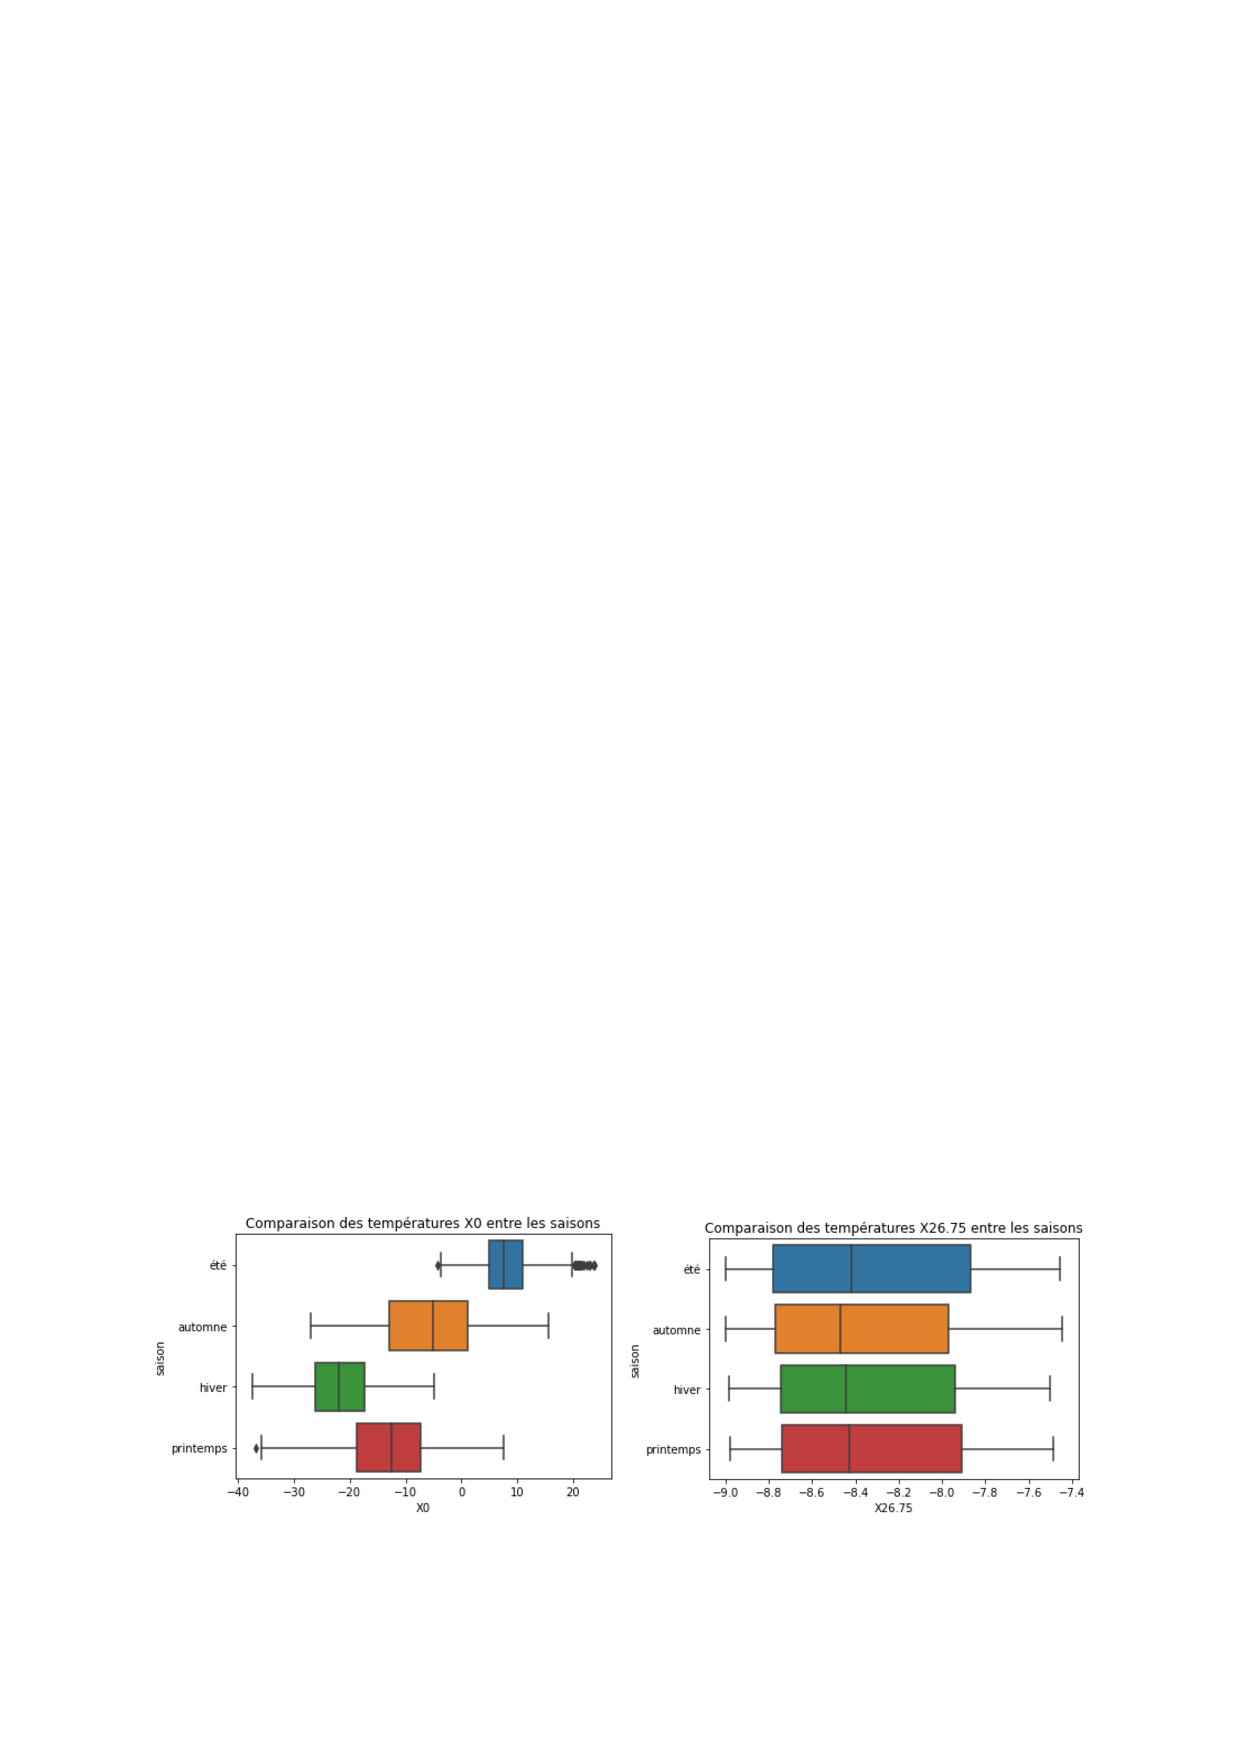
\includegraphics[scale=.8]{Saison.pdf}\end{center}

\end{figure} Estimer l'épaisseur de la couche active (voir aussi les données \texttt{activelayers.csv}).
\item
Séries temporelles (attention les deux périodes sans mesures vont poser des problèmes techniques). On pourra tester la qualité de ce modèle en prévision (par exemple en oubliant la dernière année).
\item
Modèle de régression (cf. suggestion d'exercice ci-dessous).
\end{itemize}

\newpage

\subsection*{Exercice: Modèle de régression linéaire}

\begin{enumerate}
\item Charger la base de données  \texttt{borehole\_Samoylov\_byday.csv} et représenter sur un même graphe par profondeur les  températures en fonction du temps. Que remarque-t-on?
\item
Créer une variable $D$ qui compte le nombre de jours écoulés depuis le 24-08-2006. L'avantage d'introduire une telle variable est de prendre en compte plus facilement les deux périodes sans mesures. La base de données contient aussi 6 valeurs manquantes ('NA') que nous allons supprimer.\end{enumerate}


On considère le modèle linéaire suivant: soit  $N\in \mathcal P$ (on considère un modèle linéaire par profondeur)
$$ XN_{j} = \beta_{N,0}+\beta_{N,1} D_{j}+\beta_{N,2}\cos\left(\frac{2\pi D_{j}}{365}\right)+\beta_{N,3}\sin\left(\frac{2\pi D_{j}}{365}\right)+\varepsilon_{j},\quad 1\le j\le 5147.$$
\begin{enumerate}\item[3.] Expliquer le choix de ce modèle. 
\item[4.] Implémenter ce modèle et commenter les résultats. On pourra interpréter, en fonction de la profondeur, la qualité d'ajustement du modèle aux observations et  les coefficients $\hat \beta_{1,N}$ estimés. 
\item[5.]  Donner, par profondeur, l'augmentation annuelle moyenne de température. On donnera à chaque fois un intervalle de confiance et on regardera où se trouve la valeur 0 par rapport à cet intervalle.  Mettre en regard ces résultats avec l'augmentation observée sur un siècle du pergélisol au niveau mondial.
\item[6.]  Etudier la qualité de ce modèle en prévision. Pour cela on pourra par exemple refaire tourner le modèle en laissant de coté une année complète, prédire cette année avec les coefficients estimés et calculer l'erreur de prévision associée.
\end{enumerate}

\textit{Pour aller plus loin: regarder si l'augmentation de température est homogène ou non sur les différentes profondeurs.}

	
	
	
	
 
 \subsection*{Exercice: Tests multiples}


\begin{enumerate}
\item
Charger les données \texttt{borehole\_Samoylov\_byday.csv} et effectuer quelques statistiques descriptives.
%\item
%Tracer ces séries temporelles et un boxplot pour chaque variable. Que remarque-t-on?
%\item
%Faire une classification non supervisée  sur les variables quantitatives, individus = dates, variables = différentes profondeurs. Combien de classes garder? Comparer les différentes classes, que remarque-t-on?
%\item
%Faire une ACP sur ces variables, combien d'axes faut-il garder? Sur le premier plan de l'ACP tracer le nuage de point, colorer les individus selon les classes obtenues à la question précédente.
\item Faire une série de  tests d'égalité des températures moyennes en comparant chacune des années deux à deux à différentes profondeurs. 

Comme on réalise de nombreux tests cela engendre un nombre de faux positifs important. 
Il existe de nombreuses méthodes pour contrôler le nombre de faux positifs,
 on va faire une correction de Bonferroni (on rejette l'hypothèse nulle au niveau $\alpha/N$ où $N$ est le nombre de tests effectués, ici $16\times16$ et $\alpha$ le niveau souhaité, $5\%$ en général, afin d'avoir un niveau global de $\alpha$ sur l'ensemble des tests). 
 
\item
Interpréter les résultats.
 


\end{enumerate}

\textit{Pour aller plus loin: Changer la correction du test multiple, regarder par exemple la correction de Benjamini Hochberg.}

	
	


	\subsection*{Pour aller plus loin}
	
	On dispose aussi de données multi-site qui peuvent être intéressante pour un TP plus poussé (cf. TP modèle linéaire mixte) ou un projet. Sur différents sites (plus de 200) on dispose aussi de données de températures du sol à différentes profondeurs, mais les dates auxquelles sont récoltées les données ou les profondeurs considérées varient d'un site à l'autre.  Cela permet aussi de voir du pergélisol de montagne.
		On dispose de plus 	de variables explicatives additionnelles (latitude, longitude, altitude, inclinaison du sol, faune,...).
	
	
	
	\newpage

\section{Base de données  \texttt{activelayers.csv}}
\paragraph{Présentation de la base de données} Les données proviennent du site 

\begin{center}\url{http://gtnpdatabase.org/}\end{center}




L'épaisseur  de la couche active a été mesurée par sondage du sol. Les  données sont récoltées annuellement (environ à la fin de l'été, période où la couche dégelée est maximale) et ont été obtenues de la fa\c con suivante: sur un maillage régulier : un carré de 10, 100 ou 1000 mètres de coté,  121 mesures régulièrement espacées, le sol est sondé jusqu'à atteindre la couche gelée et la profondeur (en cm) est enregistrée. Cette opération est effectuée 2 fois en chaque point du maillage.

Pour plus simplicité les valeurs par année et par site des 121 points de mesure sont résumées par les statistiques suivantes:
 \texttt{Moyenne,
 Variance,
 Minimum,
 Maximum,
 Premier quartile,
 Médiane,
 Troisième quartile.}
Pour chaque site, d'autres variables complémentaires sont aussi disponibles:
 \texttt{latitude, longitude, altitude, zone de permafrost, pente, type de végétation}.\\


 Dans la base de données \texttt{activelayers.csv} ces données sont disponibles pour 84 sites différents pour les années 1996 à 2019. La période 1969 à 1996 contenait moins de 5 sites et a donc été mise de coté, et les années 2020 et 2021 aussi pour les mêmes raisons. Txoutes les valeurs négatives sont considérées comme NA (dans cet ensemble de données, les valeurs NA sont généralement codées sous la forme -999).
 
 
 

	
\end{document}



\paragraph{Epaisseur de la couche active du pergélisol}\footnote{\emph{Fichier ActLayerLM.py, Exercice de  régression linéaire simple, en exercice de régression multiple, foret aléatoire... Dernière question test d'égalité des moyennes.}}
On travaille sur des données temporelles où en différents sites géographiques, l'épaisseur  de la couche active a été mesurée par sondage du sol. Les  données sont récoltées annuellement (environ à la fin de l'été, période où la couche dégelée est maximale) qui ont été obtenues de la fa\c con suivante: sur un maillage régulier : un carré de 10, 100 ou 1000 mètres de coté,  121 mesures régulièrement espacées le sol est sondé jusqu'à atteindre la couche gelée et la profondeur (en cm) est enregistrée. Cette opération est effectuée 2 fois en chaque point du maillage.

 Dans la base de données \texttt{activelayers.csv} ces données sont données pour 84 sites différents pour les années 1996 à 2019. Des données sont disponibles pour les 1969 à 1996, mais comme il y avait moins de 5 sites ces données ont été mises de coté, et les années 2020 et 2021 aussi pour les mêmes raisons. 
 
Sur les différents sites, ou au sein d'un site, les données n'ont pas été  récolté exactement à la même date d'une année sur l'autre ce qui ajoute de la variabilité dans les mesures. Cette variabilité est corrigée en faisant une 
 
 
 Pour plus simplicité les valeurs par année et par site des 121 points de mesure sont résumées par les statistiques suivantes:
 Moyenne,
 Variance,
 Minimum,
 Maximum,
 Premier quartile,
 Médiane,
 Troisième quartile.
Pour chaque site, d'autres variables complémentaires sont aussi disponibles:
latiture, longitude, altitude, zone de permafrost, pente, type de végétation

\begin{enumerate}
\item Créer une base de données qui pour le Minimum, le
 Maximum, la
 Médiane calcule la valeur moyenne par an. Représenter sur un même graphe ces trois courbes. Que remarque-t-on?
 \item
 On va pour la médiane ajuster un modèle linéaire en la régressant sur le temps.
Interpréter les résultats obtenus.
 Que peut-on en conclure?
 \item
Tester si l'année  1996 était celle où la couche active était minimale. 
\item
On pourra faire de même avec les autres années.
\end{enumerate}
